\subsection{Обработка звука}

\begin{frame}{Звуковая подсистема Linux}
  Виды звуковых подсистем Linux:

  \begin{enumerate}
    \item ALSA --- Advanced Linux Sound Architecture, Продвинутая звуковая архитектура Linux;
    \item OSS --- Open Sound System, Открытая звуковая система.
  \end{enumerate}
\end{frame}

\begin{frame}{ALSA}
  Ключевые особенности ALSA:

  \begin{enumerate}
    \item Эффективная поддержка всех типов звуковых интерфейсов, от любительских до профессиональных многоканальных интерфейсов;
    \item Полностью модульные звуковые драйвера;
    \item Полнодуплексная работа;
    \item Поддерживающие многопроцессорность и драйверы с потоковой безопасностью;
    \item Открытая библиотека для упрощения разработки программного обеспечения и обеспечения высокоуровневого функционала;
  \end{enumerate}
\end{frame}

\begin{frame}{PCM}
  Импульсно-кодовая модуляция (PCM)

  \begin{figure}[H]
    \centering
    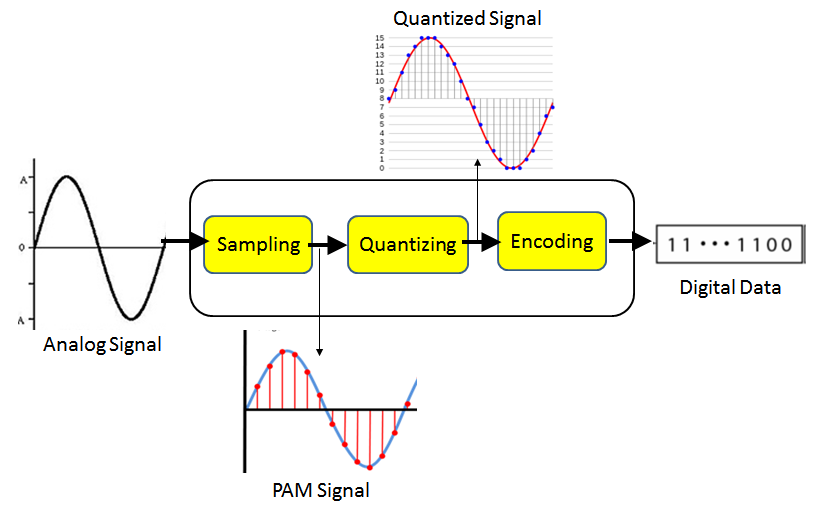
\includegraphics[width=0.65\textwidth]{assets/images/PCM.png}
    \label{img:sound__PCM}
  \end{figure}
\end{frame}

\begin{frame}{aplay, arecord}
  Необходимо указать:
  
  \begin{enumerate}
    \item Формат выходного/входного файла (по-умолчанию wav);
    \item Формат данных, или битовая глубина (по-умолчанию U8 --- беззнаковое 8-битное);
    \item Количество каналов (по-умолчанию 1);
    \item Устройство, с которого происходит запись, или на котором звуковая дорожка должна проигрываться (по умолчанию устройство, указанное в файле конфигурации ALSA);
    \item Частоту дискретизации (по-умолчанию 8 кГЦ);
    \item Файл для вывода/ввода данных.
  \end{enumerate}
\end{frame}